\documentclass[11pt, oneside]{article} 
\usepackage{geometry}
\geometry{letterpaper} 
\usepackage{graphicx}
	
\usepackage{amssymb}
\usepackage{amsmath}
\usepackage{parskip}
\usepackage{color}
\usepackage{hyperref}

\graphicspath{{/Users/telliott_admin/Dropbox/Tex/png/}}
% \begin{center} 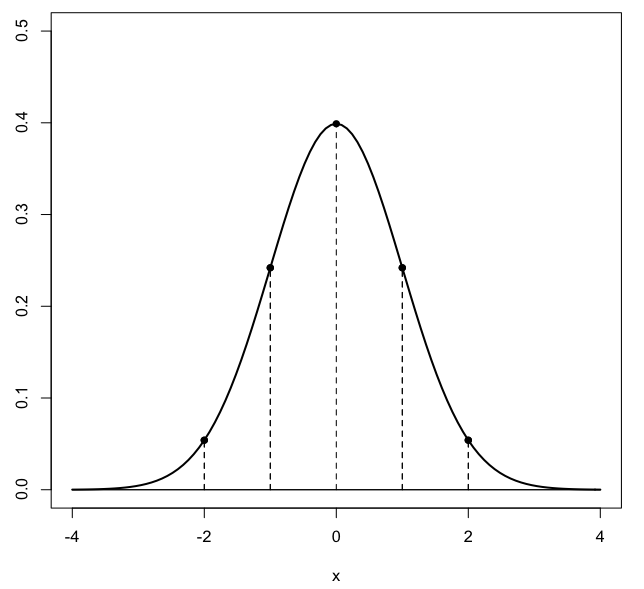
\includegraphics [scale=0.4] {gauss3.png} \end{center}

\title{Galois field $2^3$}
\date{}

\begin{document}
\maketitle
\Large

A group is about addition, a ring is about addition plus multiplication, and both satisfy various algebraic properties like closure, associativity and so on.  A field is a ring with the important distinction that each element of the field has a multiplicative inverse.

As you might guess, a finite field is a field with a finite number of elements.  The order of a finite field is the number of elements in the field.  

A familiar type of finite field can be constructed with order equal to a chosen prime number.  $Z_7$ is such a field, constructed using standard addition and multiplication, modulo 7.  

\subsection*{prime powers}
Rather than being a prime number, alternatively the order can be a prime power, that is, an integer power of a prime.  Wikipedia says that there are no other examples of finite fields beyond these two types.

In cryptography we are most interested in the field GF($2^8$), but to make the arithmetic easier, we start by exploring GF($2^3$).

The usual way to explain the construction is to talk about polynomials of the form
\[ ax^2 + bx + c \]
where the cofactors are either $0$ or $1$ (that's the $2$ part of the field's designation).  

These are the seven field elements:

\[ 1 \]
\[ x \]
\[ x + 1 \]
\[ x^2 \]
\[ x^2 + 1 \]
\[ x^2 + x \]
\[ x^2 + x + 1 \]

Unlike with $Z$, for GF($2^3$), $0$ is not an element.

GF($2^n$) has, not $2^n$ elements, but $2^{n}-1$.

The rules for arithmetic are those we've already practiced.  Addition is XOR with no carry and multiplication is polynomial multiplication:
\[ (x + 1)(x + 1) = x^2 + x + x + 1 \]
followed by the XOR addition rule:
\[ = x^2 + 1 \]

The third and final rule is that if the result of multiplication is a polynomial of degree 3 (or higher), carry out "division" by an \textbf{irreducible polynomial} until the result is of degree 2 or less.  There are two possible choices for the special polynomial:
\[ x^3 + x^2 + 1 \]
\[ x^3 + x + 1 \]

We'll see how these are arrived at in the next section.  

For example
\[ x (x^2) = x^3 \]
\[ x^3 \ \text{mod}\  (x^3 + x + 1) = x + 1 \]

A nice trick for doing this is to use the binary equivalent:
\begin{verbatim}
1000 = x^3
1011 = x^3 + x + 1
----
0011
\end{verbatim}

The result is $x + 1$, as we will repeatedly verify. 

\textbf{Notice that even though $1000$ is smaller than $1011$ in binary, we still do the XOR operation, because $1000$ is of degree 3.}

Continue doing XOR until the result is of degree 2 or less.  For example, with $x^4$ we must promote $m$ by multiplying by $10 \times 1011 = 10110$:

\begin{verbatim}
10000 = x^4
10110 = x^4 + x^2 + x
-----
00011 = x^2 + x
\end{verbatim}

\[ x^4 = x^2 + x \]

Multiplication in the binary format is a left-shift.  $2x$ is just left-shift one place.   $4x$ is left-shift two places..  

$3x$ is first $2x$, then XOR with $1x$, the original number.

Now consider 
\[ (x^2 + x + 1)(x^2 + 1) = x^4 + x^3 + x + 1 \]

One approach is

\begin{verbatim}
00101 = x^2 + 1
00111 = x^2 + x + 1
------
00101
01010
10100
-----
11011
1011  (mod) x^4 + x^2 + x 
----
01101
 1011 (mod) x^3 + x + 1
 ----
 0110
 \end{verbatim}
 
 It bears repeating that in these fields \emph{multiplication is not repeated addition} and \emph{division is not repeated subtraction (addition)}.
 
We could be tempted to do repeated XOR with the polynomial $x^3 + x + 1$.  This doesn't work.  

Here, in a different example, it's obvious:

\begin{verbatim}
  101
  100
-----
10100
 1011 (mod) x^3 + x + 1
-----
11111
\end{verbatim}

And now what?  Repeating the XOR just gives 10100 again.

Instead we must start by promoting $x^3 + x + 1$ to the degree required.  In the original problem, multiply by $x = 10$.

\begin{verbatim}
11011
1011  (mod) x^4 + x^2 + x 
----
01101
 1011 (mod) x^3 + x + 1
 ----
 0110
 \end{verbatim}

The answer is 
\[ (x^2 + x + 1)(x^2 + 1) \]
\[ = x^4 + x^3 + x + 1 \]
\[ = x^2 + x \] 

There's another approach which is worth mentioning.  We can take the intermediate result
\[ = x^4 + x^3 + x + 1 \]

and substitute for $x^4 = x^2 + x$ as well as $x^3 = x + 1$ from above
\[ = x^2 + x + x + 1 + x + 1 \]
\[ = x^2 + x \]

\subsection*{irreducible polynomials}
We will want to find polynomials that do not have factors, that cannot be arrived at by multiplying together two polynomials.

For this multiplication we are not using the special rule mod rule yet, we are not working in the field.  We are just looking.  However, we do use XOR addition.

The degree 2 or smaller polynomials are
\[ 1 \]
\[ x + 1 \]
\[ x \]

Multiplying by $1$ doesn't give anything new.

To go to degree 2 multiply 
\[ x \cdot x = x^2 \]
\[ x(x + 1) = x^2 + x \]
\[ (x + 1)(x + 1) = x^2 + 1 \]

There is one more degree 2 polynomial that is not generated by this procedure:
\[ x^2 + x + 1 \]

Since $x^2 + x + 1$ has no "factors" in the field (it was not produced by exhaustive multiplication of the field elements), it is irreducible, which is (somewhat) analogous to being prime.  It has no factors.  

It can be used to form the field GF($2^2$), which has three elements.  We are going to skip that for now.

Next, by multiplying all pairwise combinations of degree 1 with degree 2 to form degree 3 polynomials, we find eight results and six which are unique.

\[ x(x^2) = x^3 \]
\[ x(x^2 + 1) = x^3 + x  \]
\[ x(x^2 + x) = x^3 + x^2 \]
\[ x(x^2 + x + 1) = x^3 + x^2 + x  \]

\[ (x+1)(x^2) = x^3 + x^2   \]
\[ (x+1)(x^2 + 1) =  x^3 + x^2 + x + 1 \]
\[ (x+1)(x^2 + x) = x^3 + x^2 + x^2 + 1 =  x^3 + 1 \]
\[ (x+1)(x^2 + x + 1) = x^3 + x^2 + x + x^2 + x + 1 = x^3 + 1 \]

Two polynomials of degree 3 are not produced by this method.  It is easier to see which they are if we write the results in binary:
\begin{verbatim}
1000 1010 1001
1100 1110 1111
\end{verbatim}

The two missing polynomials, $1011$ and $1101$, are the irreducible ones.
\[ x^3 + x + 1 \]
\[ x^3 + x^2 + 1 \]

We might choose either of these to form the field GF($2^3$).  

We chose the first one, above.  Once we've made the choice, we must stick with it, to produce consistent results.

\subsection*{multiplication table}
Constructing a multiplication table at this scale (7 x 7) is a bit of a pain, but it's a useful exercise.  Start by re-computing the modulus results for $x^3$ and $x^4$:

\begin{verbatim}
1000 x^3
1011
----
0011 x + 1
\end{verbatim}

$x^3$ is equal to $x + 1$ in this field, and $x^4 = x^2 + x$ because
\[ x^4 \ \text{mod} \ x^3 + x + 1 = x^2 + x \]

\begin{verbatim}
10000 x^4
10110
-----
00110 x^2 + x
\end{verbatim}

That was just a left-shift of the irreducible polynomial by one place (corresponding to multiplication by 010).

When we say:  "$x^3$ is equal to $x + 1$ in this field" we mean that anywhere $x^3$ arises it can be replaced by $x + 1$.  They are the same.

If there additional terms, say we had $x^3 + x$, the result is $x + 1$ from $x^3$ then XOR the other term(s):  here the result is 1.  Thus
\[ x^3 + x  \ \text{mod} \ x^3 + x + 1 = 1 \]

And therefore, factoring, we find that $x^2 + 1$ and $x$ are multiplicative inverses.

Let's start the table
\[ 
\begin{matrix}
1 & x & x + 1 & x^2 & x^2 + 1 & x^2 + x & x^2 + x + 1 \\
x & x^2 & . & . & . &.  & . \\
x + 1 & x^2 + x & . & . & . & . & . \\
x^2 & x + 1  & . & . & . & . & . \\
x^2 + 1 & 1  & . & . & . & . & . \\
x^2 + x & x^2 + x + 1   & . & . & . & . & . \\
x^2 + x + 1 & x^2 + 1 & . & . & . & . & . \\
\end{matrix} 
\]
The second column contains each of the elements multiplied by $x$.  For $x(x^2)$ we used the fact that $x^3 = x + 1$ as described above.

Also, $x(x^2 + x) = x^3 + x^2 = (x + 1$) XOR $x^2 = x^2 + x + 1$.  

Finally $x(x^2 + x + 1) = x^3 + x^2 + x = (x + 1) $ XOR $x^2 + x = x^2 + 1$.

Each column and each row will turn out to contain all 7 elements of the field.  
\[ 
\begin{matrix}
1 & x & x + 1 & x^2 & x^2 + 1 & x^2 + x & x^2 + x + 1 \\
x & x^2 & x^2 + x & x + 1 & 1 & x^2 + x + 1  & x^2 + 1 \\
x + 1 & x^2 + x & x^2 + 1 & x^2 + x + 1 & x^2 & 1 & x \\
x^2 & x + 1  & x^2 + x + 1 & x^2 + x & x & x^2 + 1 & 1 \\
x^2 + 1 & 1  & x^2 & x & x^2 + x + 1 & x + 1 & x^2 + x \\
x^2 + x & x^2 + x + 1   & 1 & x^2 + 1& x + 1 & x & x^2 \\
x^2 + x + 1 & x^2 + 1 & x & 1 & x^2 + x & x^2 & x + 1 \\
\end{matrix} 
\]

The same 7 elements fill each row and each column.  Every polynomial has a unique inverse, and the inverses match (of course).

Having filled out and laborious re-checked the table, it's pretty clear that polynomials are a painful way to do this sort of thing.

Instead, we can try writing binary numbers.
\newpage
\begin{verbatim}
001   010   011   100   101   110   111
010   100   110
011   110   101
100   011
101
110
111
\end{verbatim} 

In filling out the second column, we have reached the first division operation.
\[ 100 * 010 = 1000 \rightarrow 011 \]
\[ 101 * 010 = 1010 \rightarrow 001 \]
It is very fast with pen and paper and not at all error-prone.

Two points:  first, this is one way to find multiplicative inverses for a field like GF($2^3$):  exhaustive calculation.  

However, it is not practical for GF($2^8$) with 65,000+ multiplications.

Second, the reason for choosing an irreducible polynomial becomes clear:  multiplication \emph{must not} produce $0$, because $0$ is not in the field.

\subsection*{Other methods}
What about other approaches?  There are at least three.

The one we use extensively elsewhere (in code) is based on knowledge that \textbf{0x03} is a primitive element or generator of the field GF($2^8$), which is to say that (\textbf{0x03})$^8 =$ \textbf{0x03}.  When wikipedia talks about the $q-1$ root of unity, this is what they refer to (\textbf{0x03})$^7 =$ \textbf{0x01}).

We would need to find a generator of the field GF($2^3$).

By self-multiplying, we produce a table of powers, and then by inverting the table produce discrete logarithms.  Subsequently, find logs which sum to the right number (i.e. 7).  We'll see that below.

The second method is the extended Euclidean algorithm.  And the third is the one we take up next.

Suppose we want to find the multiplicative inverse of $x^2 + x$ in GF($2^3$).  Write a general polynomial
\[ (x^2 + x) (ax^2 + bx + c) \]
\[ = ax^4 + bx^3 + cx^2 + ax^3 + bx^2 + cx \]
group like terms:
\[ = ax^4 + (b + a)x^3 + (c + b)x^2 + cx \]

Now, just substitute for the values of $x^4$ and $x^3$ mod the irreducible polynomial $x^3 + x + 1$, namely
\[ =  a(x^2 + x) + (b + a)(x + 1) + (c + b)x^2 + cx \]
so again re-group to obtain
\[ = (a + b + c)x^2 + (a + b  + a + c)x + (a + b) \]
\[ = (a + b + c)x^2 + (b  + c)x + (a + b) \]
The source 

\url{https://math.stackexchange.com/questions/2357753/multiplicative-inverse-in-gf23-without-euclidiean-algorithm}

has
\[ = (b + c - a)x^2 + (c - b)x + (a + b) \]
but subtraction is the same as addition, so these are equivalent.

Our goal is that the product should be equal to $1$, that is to the polynomial with coefficients $(0,0,1)$ thus:
\[ a + b + c = 0 \]
\[ b + c = 0 \]
\[ a + b = 1 \]

Subtracting the second from the first, it is clear that $a = 0$.  

If we supposed that $a = 1$ then we would have $b = 0, c = 0$ and $1 + 0 + 0 = 0$, a contradiction.  Hence $a = 0$.

Then, $b = 1$ and $c = 1$ also, since $1 + 1 = 0$.  Therefore, the inverse should be $x + 1$.  Check it:
\[ (x^2 + x)(x + 1) = x^3 + x^2 + x^2 + x = x^3 + x \]
Divide by $x^3 + x + 1$ (or just add $x + 1$) and obtain $1$ as the answer.  It checks.

\subsection*{generators}

Some elements are generators, some are not.  I tried $011$ because it works with GF($2^8$):

\begin{verbatim}
0011
0011
----
0011
0110
----
0101  =>  0101
===========
0101
0011
----
0101
1010
----
1111
1011
----
0100  =>  101, 100
===========
0100
0011
----
0100
100
----
1100
1011
----
0111  =>  101, 100, 111
...
\end{verbatim}
Rather than go all the way around with this method, let's try polynomials.  The last element we got was $x^2 + x + 1$.  The generator is $x + 1$ so the next round is
\[ (x + 1)(x^2 + x + 1) = x^3 + x^2 + x + x^2 + x + 1 \]
Canceling and substituting for $x^3$:
\[ = (x + 1) + 1 = x \]
Then
\[ (x + 1)(x) = x^2 + x \]
That's five.

\[ (x + 1)(x^2 + x) = x^3 + x^2 + x^2 + x \]
\[ = (x + 1) + x = 1\]

Finally
\[ (x + 1)(1) = x + 1 \]

That's all seven, that's all we need.  Here they are, along with their logarithms.

\begin{verbatim}
011, 101, 100, 111, 010, 110, 001, 011
  1,   2,   3,   4,   5,   6,   7,   8
\end{verbatim}
Since the generator to the $0$ power is equal to the generator to the $7$ power, we need the logs to sum to $7$.  

As an example, the log of $x^2 + x = 110$ is $6$.  The log of its multiplicative inverse must therefore be $1$, which corresponds to $011$.  We showed already that $011 = x + 1$ is the correct value.

\subsection*{Kak note}
According to Kak, the generator g is that element that symbolically satisfies 

\[ g^3 + g + 1 = 0 \]

which implies that
\[ g^3 = -g - 1 = g + 1\]

If the irreducible polynomial for GF($2^3$) has been chosen as $g^3 + g + 1$, we see the parallel.

The elements are powers of the generator
\begin{verbatim}
g^0 = 1
g^1 = g
g^2 = g^2
g^3 = g + 1
g^4 = g(g^3) = g^2 + g
g^5 = g(g^4) = g^3 + g^2 = g^2 + g + 1
g^6 = g(g^5) = g^3 + g^2 + g = g^2 + 1
g^7 = g(g^6) = g^3 + g = 1
\end{verbatim}

I am not quite sure yet of the difference between this "symbolic" manipulation of the generator and the arithmetic mod m that we do with an actual generator.

We found that binary $11 = 3$ is a generator for GF($2^3$) with $1011$ as the irreducible polynomial.

\begin{verbatim}
011 * 001 = 0011
011 * 011 = 0101
011 * 101 = 1111 = 100 (mod 1011)
011 * 100 = 1100 = 111 (mod 1011)
011 * 111 = 1001 = 010 (mod 1011)
011 * 010 = 0110
011 * 110 = 1010 = 001 (mod 1011)
\end{verbatim}

So that's all 7:
\begin{verbatim}
001 011 101 100 111 010 110 001
\end{verbatim}

The table of logs is
\begin{verbatim}
001 011 101 100 111 010 110 001
  0   1   2   3   4   5   6   7
\end{verbatim}

Note that with the other possible choice of polynomial

\begin{verbatim}
011 * 001 = 0011
011 * 011 = 0101
011 * 101 = 1111 = 010 (mod 1101)
011 * 010 = 0110
011 * 110 = 1010 = 111 (mod 1101)
011 * 111 = 1001 = 100 (mod 1101)
011 * 100 = 1100 = 001 (mod 1101)
\end{verbatim}

That is
\begin{verbatim}
001 011 101 010 110 111 100 001
\end{verbatim}

Same elements, different order.
 
So now if we generate a table of logs:
\begin{verbatim}
001 011 101 010 110 111 100 001
  0   1   2   3   4   5   6   7
\end{verbatim}

We find that $010$ and $110$ are inverses, whereas in the first scheme 

\begin{verbatim}
010 * 101 = 1
110 * 011 = 1
\end{verbatim}

So the elements are the same, but the math including multiplicative inverses is all different.

\end{document}

